\documentclass[border=10pt]{standalone}
\usepackage{underscore}
\usepackage{tikz}
\usetikzlibrary{shapes,arrows,positioning,calc,backgrounds,matrix,fit,decorations.pathreplacing}

\newcount\index
\newcommand{\diaName}{default name}
\newcommand{\diaWidth}{10em}
\newcommand{\diaHeight}{2em}
\newcommand{\updateIndex}{\advance\index by 1\relax}
\newcommand{\lastId}{\diaName-\the\numexpr\index-1\relax}
\newcommand{\id}{\diaName-\the\index}

\newcommand{\record}[2]{
    \node[fixed node={\diaWidth}{\diaHeight},below=of \lastId,#1](\id){#2};
    \updateIndex
}
%%% environment struct
\newenvironment{struct}[3]
{
    \index=0
    \renewcommand{\diaName}{#1}
    \renewcommand{\diaWidth}{#2}
    \renewcommand{\diaHeight}{#3}
}
{
    \node[fit=(\diaName-0)(\lastId),inner sep=0pt](\diaName){};
}
%%% environment struct end


\tikzset{
    table/.style 2 args={
        draw,
        rectangle,
        inner sep=0pt,
        matrix of nodes,
        nodes in empty cells,
        nodes={
            draw,
            font=\ttfamily,
            align=center,
            text width=#1,
            outer sep=0pt,
            inner sep=0.3em,
            minimum height=1.6em
        },
        label={[align=center]90:\bf{#2}}
    },
    table/.default={10cm}{},
    right brace/.style 2 args={
        decorate,
        decoration={brace,amplitude=#1,raise=#2}
    },
    right brace/.default={8pt}{2pt},
    right note/.style={right=#1},
    right note/.default={0.3cm},
    left note/.style={left=#1},
    left note/.default={0.3cm},
    left brace/.style 2 args={
        decorate,
        decoration={brace,amplitude=#1,raise=#2,mirror}
    },
    left brace/.default={8pt}{2pt},
    right addr note/.style={right=#1},
    right addr note/.default={0.5cm},
    left addr note/.style={left=#1},
    left addr note/.default={0.5cm},
    arrow/.style={>=stealth',->},
    fixed node/.style 2 args={
        node distance=0,
        outer sep=0,
        inner sep=0,
        draw,
        font=\ttfamily,
        rectangle,
        minimum width=#1,
        minimum height=#2
    },
    title node/.style={rectangle,inner sep=1em},
    blank cell/.style={fill=white,minimum height=1cm},
    non blank cell/.style={fill=cyan!30,minimum height=#1}
}


\newcommand{\sybwd}{32em}
\newcommand{\sybht}{2em}
\newcommand{\sybleftwd}{12em}
\newcommand{\sybleftht}{5em}
\newcommand{\sybrightwd}{20em}
\newcommand{\sybrightht}{2em}

\newcommand{\methodwd}{36em}
\newcommand{\methodht}{2em}
\newcommand{\methodleftwd}{20em}
\newcommand{\methodleftht}{3em}
\newcommand{\methodrightwd}{16em}
\newcommand{\methodrightht}{4em}

\begin{document}
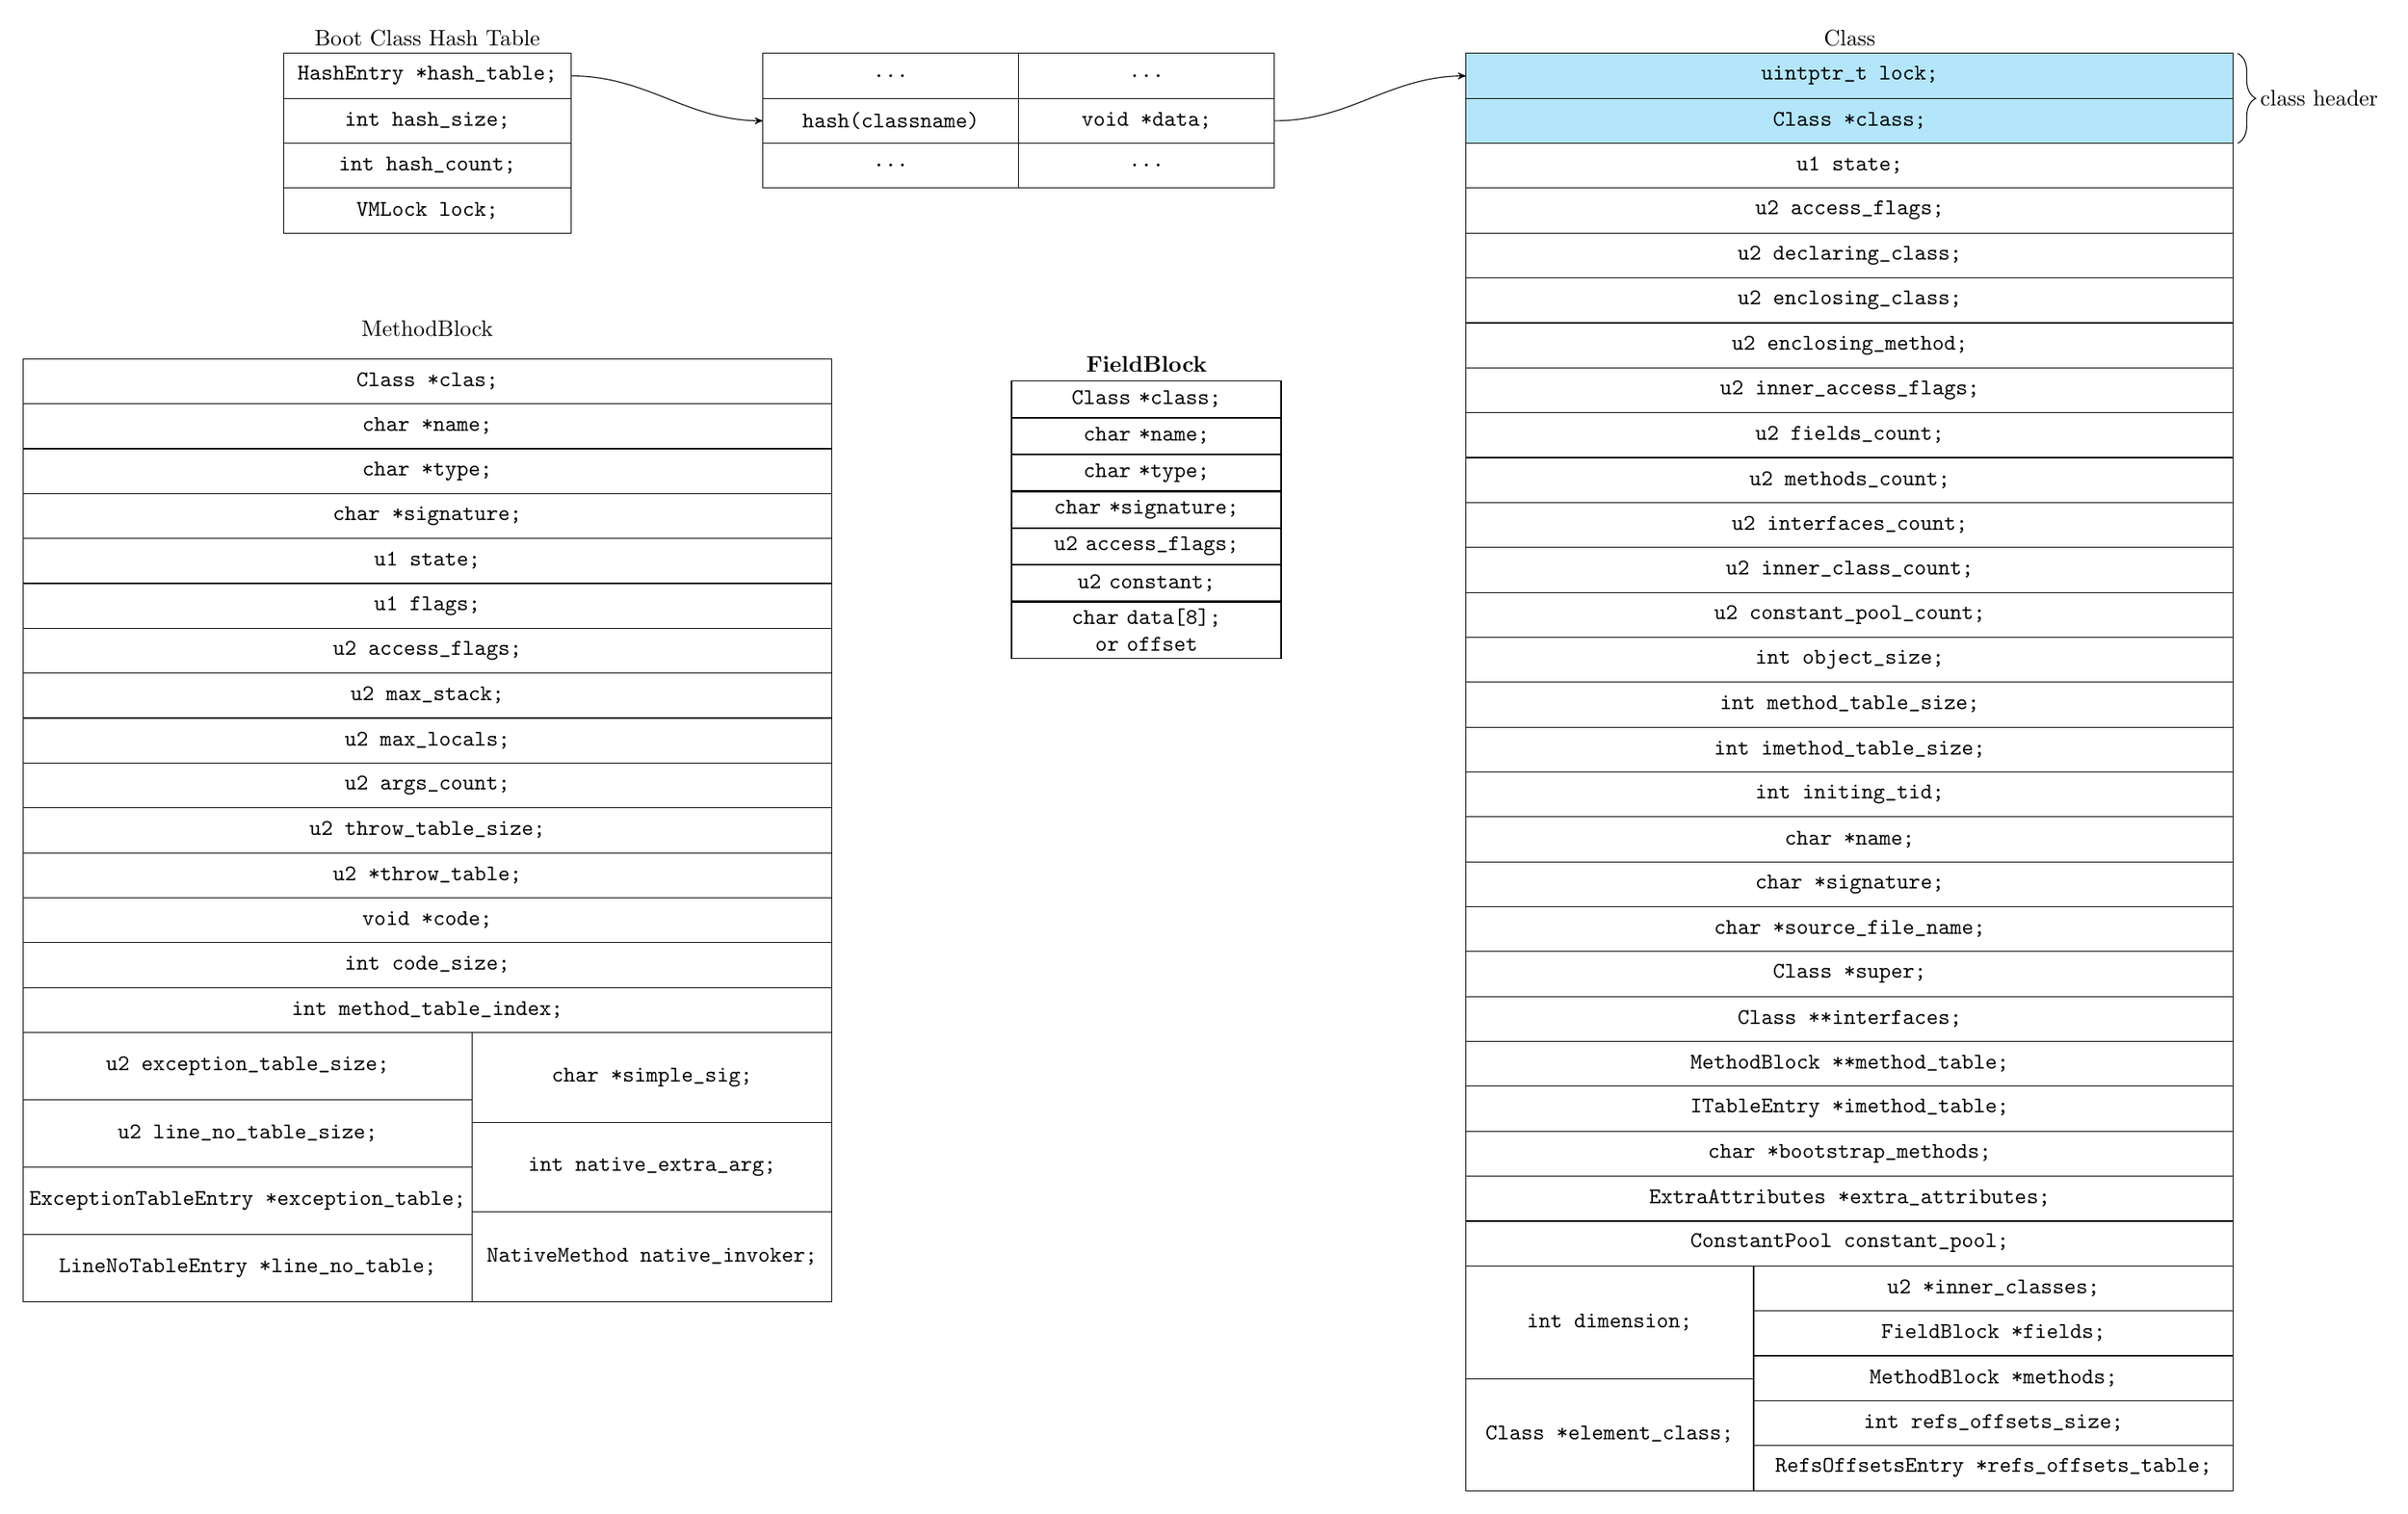
\begin{tikzpicture}

    %%% hashtable
    \begin{struct}{hashtable}{4.5cm}{2em}
        \node[fixed node={\diaWidth}{\diaHeight},label={Boot Class Hash Table}]
            (\id){HashEntry *hash_table;};\updateIndex
        \record{}{int hash_size;}
        \record{}{int hash_count;}
        \record{}{VMLock lock;}
    \end{struct}


    %%% hash data
    \begin{struct}{hashdata1}{4cm}{2em}
        \node[fixed node={\diaWidth}{\diaHeight},right=3cm of hashtable-0](\id){...};\updateIndex
        \record{}{hash(classname)}
        \record{}{...}
    \end{struct}
    \begin{struct}{hashdata2}{4cm}{2em}
        \node[fixed node={\diaWidth}{\diaHeight},right=0cm of hashdata1-0](\id){...};\updateIndex
        \record{}{void *data;}
        \record{}{...}
    \end{struct}


    %%% Class
    \begin{struct}{class}{12cm}{2em}   
        \node[fixed node={\diaWidth}{\diaHeight},label={Class},right=3cm of hashdata2-0,fill=cyan!30](\id){uintptr_t lock;};\updateIndex
        \record{fill=cyan!30}{Class *class;};
        \record{}{u1 state;};
        \record{}{u2 access_flags;};
        \record{}{u2 declaring_class;};
        \record{}{u2 enclosing_class;};
        \record{}{u2 enclosing_method;};
        \record{}{u2 inner_access_flags;};
        \record{}{u2 fields_count;};
        \record{}{u2 methods_count;};
        \record{}{u2 interfaces_count;};
        \record{}{u2 inner_class_count;};
        \record{}{u2 constant_pool_count;};
        \record{}{int object_size;};
        \record{}{int method_table_size;};
        \record{}{int imethod_table_size;};
        \record{}{int initing_tid;};
        \record{}{char *name;};
        \record{}{char *signature;};
        \record{}{char *source_file_name;};
        \record{}{Class *super;};
        \record{}{Class **interfaces;};
        \record{}{MethodBlock **method_table;};
        \record{}{ITableEntry *imethod_table;};
        \record{}{char *bootstrap_methods;};
        \record{}{ExtraAttributes *extra_attributes;};
        \record{}{ConstantPool constant_pool;};
    \end{struct}
    \begin{struct}{class-union-left}{4.5cm}{5em}
        \node[fixed node={\diaWidth}{\diaHeight},anchor=north west](\id)at(class.south west){int dimension;};\updateIndex
        \record{}{Class *element_class;};
    \end{struct}
    \begin{struct}{class-union-left}{7.5cm}{2em}
        \node[fixed node={\diaWidth}{\diaHeight},anchor=north west](\id)at(class-union-left.north east){u2 *inner_classes;};\updateIndex
        \record{}{FieldBlock *fields;};
        \record{}{MethodBlock *methods;};
        \record{}{int refs_offsets_size;};
        \record{}{RefsOffsetsEntry *refs_offsets_table;};
    \end{struct}


    %%% Field
    \matrix (fieldblock) [table={4cm}{FieldBlock},below=3cm of hashdata1,xshift=4cm] {
        ||{Class *class;}\\
        ||{char *name;}\\
        ||{char *type;}\\
        ||{char *signature;}\\
        ||{u2 access_flags;}\\
        ||{u2 constant;}\\
        ||{char data[8]; or offset}\\
    };


    %%% MethodBlock
    \node[rectangle,inner sep=1em,below=1cm of hashtable](method title){MethodBlock};
    \node[fixed node={\methodwd}{\methodht},below=of method title](m1){Class *clas;};
    \node[fixed node={\methodwd}{\methodht},below=of m1](m2){char *name;};
    \node[fixed node={\methodwd}{\methodht},below=of m2](m3){char *type;};
    \node[fixed node={\methodwd}{\methodht},below=of m3](m4){char *signature;};
    \node[fixed node={\methodwd}{\methodht},below=of m4](m5){u1 state;};
    \node[fixed node={\methodwd}{\methodht},below=of m5](m6){u1 flags;};
    \node[fixed node={\methodwd}{\methodht},below=of m6](m7){u2 access_flags;};
    \node[fixed node={\methodwd}{\methodht},below=of m7](m8){u2 max_stack;};
    \node[fixed node={\methodwd}{\methodht},below=of m8](m9){u2 max_locals;};
    \node[fixed node={\methodwd}{\methodht},below=of m9](m10){u2 args_count;};
    \node[fixed node={\methodwd}{\methodht},below=of m10](m11){u2 throw_table_size;};
    \node[fixed node={\methodwd}{\methodht},below=of m11](m12){u2 *throw_table;};
    \node[fixed node={\methodwd}{\methodht},below=of m12](m13){void *code;};
    \node[fixed node={\methodwd}{\methodht},below=of m13](m14){int code_size;};
    \node[fixed node={\methodwd}{\methodht},below=of m14](m99){int method_table_index;};

    \node[fixed node={\methodleftwd}{\methodleftht},anchor=north west] (m100) at (m99.south west) {u2 exception_table_size;};
    \node[fixed node={\methodleftwd}{\methodleftht},below=of m100](m101){u2 line_no_table_size;};
    \node[fixed node={\methodleftwd}{\methodleftht},below=of m101](m102){ExceptionTableEntry *exception_table;};
    \node[fixed node={\methodleftwd}{\methodleftht},below=of m102](m103){LineNoTableEntry *line_no_table;};

    \node[fixed node={\methodrightwd}{\methodrightht},anchor=north west](m200) at (m100.north east) {char *simple_sig;};
    \node[fixed node={\methodrightwd}{\methodrightht},below=of m200](m201){int native_extra_arg;};
    \node[fixed node={\methodrightwd}{\methodrightht},below=of m201](m202){NativeMethod native_invoker;};

    %%% lines
    \draw[arrow] (hashtable-0.east) to[out=0,in=180] (hashdata1-1.west);
    \draw[arrow] (hashdata2-1.east) to[out=0,in=180] (class-0.west);
    \draw[right brace] (class-0.north east) -- node[right note]{class header} (class-1.south east);
\end{tikzpicture}
\end{document}


